
\documentclass{DocBleu}
\usepackage{pgfplots}
\usetikzlibrary{positioning,arrows.meta,calc}

\usepackage{multirow}
\usetikzlibrary{arrows}
\usetikzlibrary{calc,trees,positioning,arrows,chains,shapes.geometric,%
decorations.pathreplacing,decorations.pathmorphing,shapes,%
matrix,shapes.symbols,plotmarks,decorations.markings,shadows}\newcommand{\Prob}{\textbf{\textsf{\textup{P}}}}  % Probability over a set
\newcommand{\prob}{\textbf{\textsf{\textup{p}}}}  % Probability density


\begin{document}
\chapter{Utilisation de réseaux existants}
\PartialToC
%%%%
Depuis la fin des années 90, de nombreux réseaux profonds ont vu le jour et se sont complexifié, diversifié, pour répondre à des problèmes de plus en plus vastes. \cite{Canziani16} propose une analyse comparative de ces réseaux et décrit en particulier leurs performances en fonction du nombre d'opérations (figure \ref{F:compar}).

Nous présentons dans la suite cinq réseaux profonds classiques. Nous montrons ensuite comment les utiliser directement, ou comment les adapter pour répondre à une problématique précise, en lien avec leur utilisation originale ou non. Nous introduisons enfin une  manière d'apprendre  un réseau à partir de  peu  de données.

\begin{figure}[hbtp!]
\centering
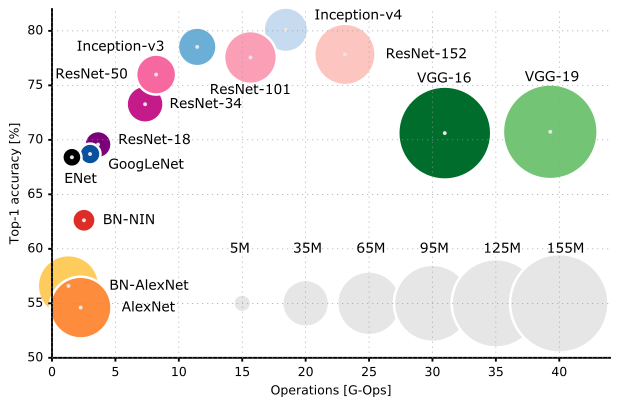
\includegraphics[scale=.7]{images/comparaison.png}
\caption{Précision en fonction du nombre d'opérations nécessaire pour un calcul en passe avant. La taille des blobs est proportionnelle au nombre de paramètres du réseau (source : \cite{Canziani16})}
\label{F:compar}
\end{figure}

\section{Quelques réseaux profonds classiques}

Les cinq réseaux présentés ici ont prouvé leur efficacité, notamment lors des compétitions organisées depuis 2010 sur une base de données d'images nommée \href{http://www.image-net.org/}{ImageNet}. Initiée à l'Université de Stanford, cette base de données comporte aujourd'hui plus de 14 millions d'images, classées en 21841 catégories (avions, voitures, chats,...). Dans les compétitions ILSVRC ( ImageNet Large Scale Visual Recognition Challenge), les chercheurs se voient proposer une extraction de 1,2 millions d'images, catégorisées en 1000 classes, et le gagnant est celui qui atteint la meilleure précision de reconnaissance sur les 5 premières classes (top-5). \\


\subsection{AlexNet}
En 2012,  Krizhevsky et al \cite{Krizhevsky12} remportent ILSVRC avec un taux de reconnaissance de 84.6\%, en utilisant AlexNet, un réseau convolutif composé de 5 couches de convolution et de pooling, suivies de 3 couches complètement connectées (figure \ref{F:Alexnet}). 
\begin{figure}[hbtp!]
\centering
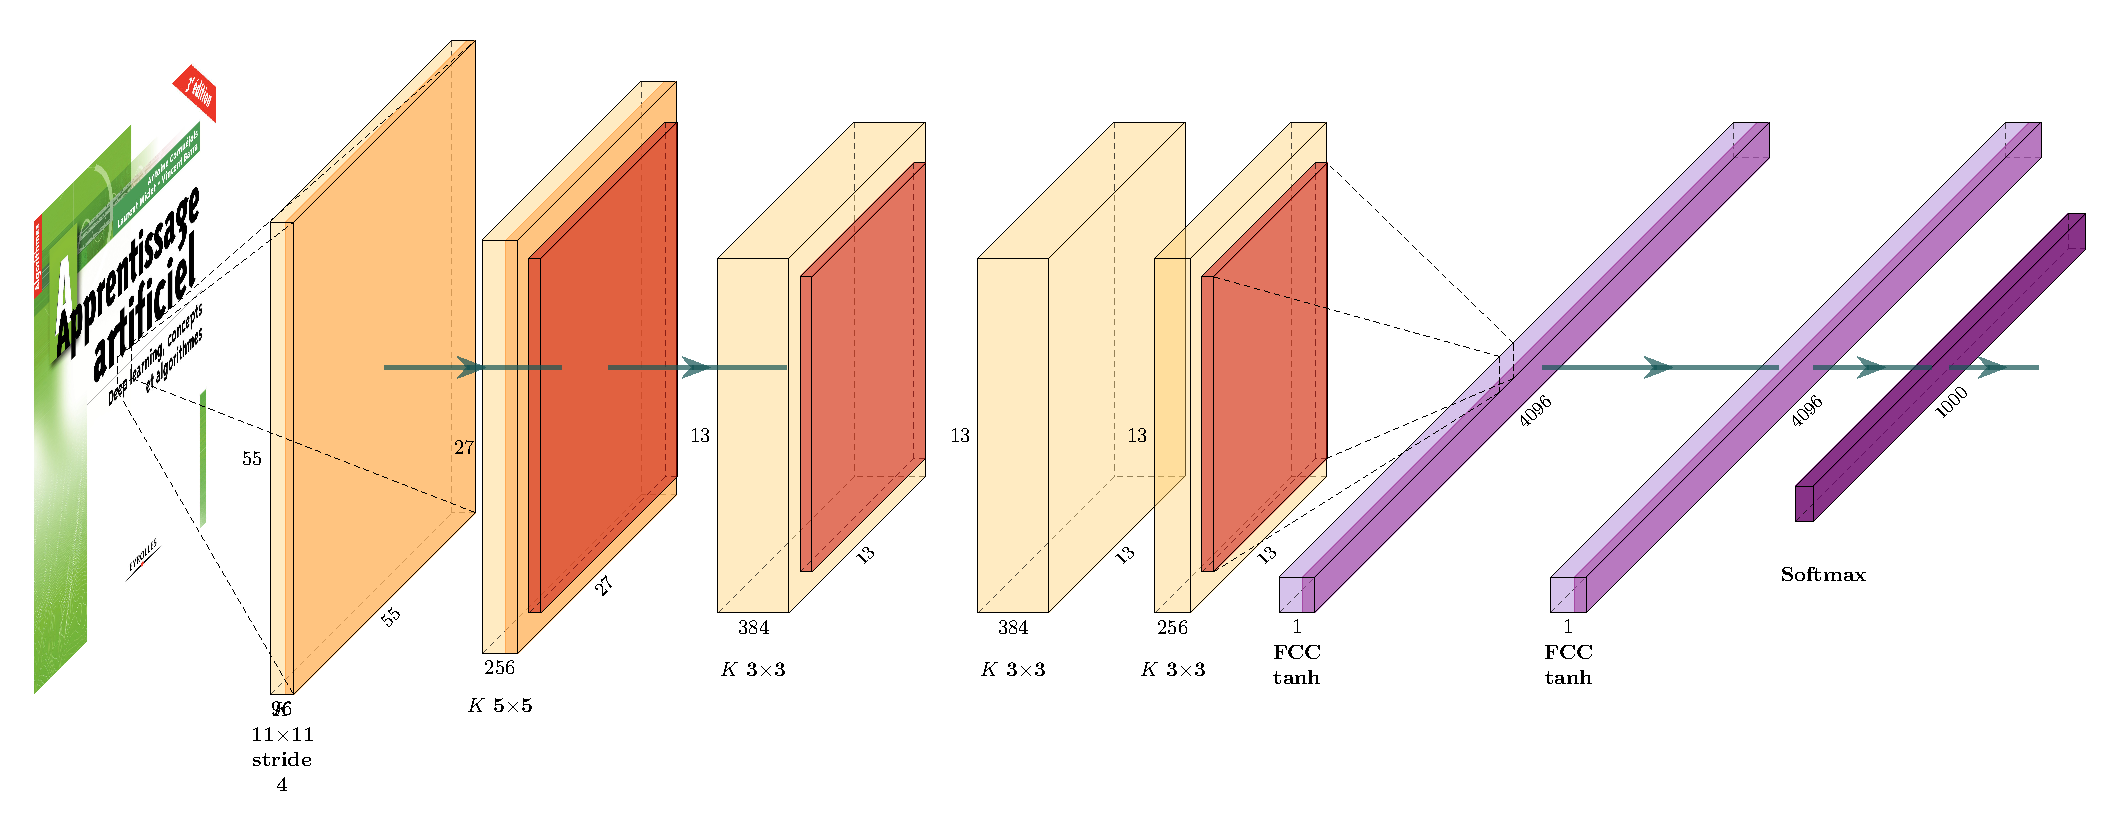
\includegraphics[width=\textwidth]{images/AlexNet.pdf}
\caption{Architecture du r\'eseau AlexNet. Les couches de convolution et d'activation sont en orange clair, les couches d'agr\'egation en orange fonc\'e. Les couches compl\`etement connect\'ees sont en violet.}
\label{F:Alexnet}
\end{figure}



Si la profondeur du réseau reste faible, le nombre de paramètres était déjà important. En regardant uniquement la première couche de convolution, on constate que :
\begin{itemize}
\item l'entrée est composée d'images 227$\times$227$\times$3
\item les filtres  de convolution sont de taille 11
\item le pas de convolution (stride) est de 4
\end{itemize}
Ainsi la sortie de la couche de convolution est de taille 55$\times$55$\times$96=290 400 neurones, chacun ayant 11$\times$11$\times$3=363 poids et un biais.  Cela implique, sur cette couche de convolution seulement, 105 705 600 paramètres à ajuster.\\
Ce réseau, amélioration d'un réseau existant (LeNet), apportait de nombreuses contributions, comme l'utilisation de couches ReLU, de dropout, ou du GPU (NVIDIA GTX 580) pendant la phase d'entraînement.

\subsection{VGG}
Les réseaux VGG (Visual Geometry Group, université d'Oxford) \cite{Simonyan14} ont été les premiers réseaux à utiliser de petits filtres de convolution (3$\times$3) et à les combiner pour décrire des séquences de convolution, l'idée étant d'émuler l'effet de larges champs réceptifs par cette séquence. Cette technique amène malheureusement à un nombre exponentiel de paramètres (le modèle entraîné qui peut être téléchargé a une taille de plus de 500 Mo).
VGG a concouru à ILSVRC 2014, a obtenu un taux de bonne classification de 92.3\% mais n'a pas remporté le challenge.
Aujourd'hui VGG et une famille de réseaux profonds (de A à E)  qui varient par leur architecture (figures \ref{F:VGG} et \ref{F:vgg16}). Le nombre de paramètres (en millions) pour les réseaux de A à E est 133, 133, 134, 138 et 144. Les réseaux VGG-D et VGG-E sont les plus précis et populaires.

\begin{center}
\begin{figure}[hbtp!]
\centering
\begin{tabular}{|c||c||c||c||c||c|}
\hline
\bf{}A&\bf{A-LRN}&\bf{B}&\bf{C}&\bf{D}&\bf{E} \\ \hline
  11 couches &  11 couches &  13 couches &  16 couches &  16 couches &  19 couches \\  \hline
  \multicolumn{6}{|c|}{Entrée : image 224$\times$224 RGB} \\\hline
  \multirow{2}{*}{}conv3-64 & conv3-64 & conv3-64 & conv3-64 & conv3-64& conv3-64\\
  & LRN& conv3-64& conv3-64& conv3-64& conv3-64\\ \hline
    \multicolumn{6}{|c|}{max pooling} \\\hline
  \multirow{2}{*}{}conv3-128 & conv3-128 & conv3-128 & conv3-128 & conv3-128& conv3-128\\
  && conv3-128& conv3-128& conv3-128& conv3-128 \\\hline
    \multicolumn{6}{|c|}{max pooling} \\\hline
  \multirow{4}{*}{}conv3-256 & conv3-256 & conv3-256 & conv3-256 & conv3-256& conv3-256\\
conv3-256 & conv3-256 & conv3-256 & conv3-256 & conv3-256& conv3-256\\
  &&& conv1-256& conv3-256& conv3-256 \\
  &&&&&conv3-256 \\\hline
    \multicolumn{6}{|c|}{max pooling} \\\hline
  \multirow{4}{*}{}conv3-512 & conv3-512 & conv3-512 & conv3-512 & conv3-512& conv3-512\\
conv3-512 & conv3-512 & conv3-512 & conv3-512 & conv3-512& conv3-512\\
  &&& conv1-512& conv3-512& conv3-512 \\
  &&&&&conv3-512\\\hline
    \multicolumn{6}{|c|}{max pooling} \\\hline
  \multirow{4}{*}{}conv3-512 & conv3-512 & conv3-512 & conv3-512 & conv3-512& conv3-512\\
conv3-512 & conv3-512 & conv3-512 & conv3-512 & conv3-512& conv3-512\\
  &&& conv1-512& conv3-512& conv3-512 \\
  &&&&&conv3-512\\\hline
      \multicolumn{6}{|c|}{max pooling} \\\hline
    \multicolumn{6}{|c|}{Couche complètement connectée 4096 neurones} \\\hline
    \multicolumn{6}{|c|}{Couche complètement connectée 4096 neurones} \\\hline
    \multicolumn{6}{|c|}{Couche complètement connectée 1000 neurones} \\\hline
    \multicolumn{6}{|c|}{Classifieur softmax} \\\hline
\end{tabular}
 \caption{Architectures des réseaux VGG}
\label{F:VGG}
\end{figure}
\end{center}

\begin{figure}
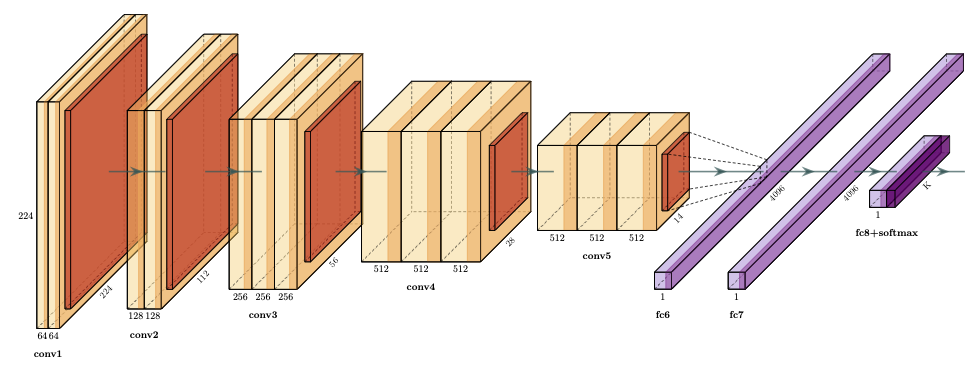
\includegraphics[width=\textwidth]{images/VGG16}
\caption{Réseau VGG16}
\label{F:vgg16}
\end{figure}


\subsection{Inception}
Inception, proposé par Google, est le premier réseau dont les performances ont été augmentées pas seulement en augmentant le nombre de couches, mais en pensant et optimisant le design et l'architecture. L'idée est ici d'utiliser plusieurs filtres, de tailles différentes, sur la même image  et de concaténer les résultats pour générer une représentation plus robuste. \\
Inception n'est pas un réseau, c'est une famille de réseaux :  Network in Network \cite{Lin13}, Inception V1 \cite{Szegedy14}, Inception V2 \cite{Szegedy15}, Xception \cite{Chollet16},...\\
L'idée du premier réseau (figure \ref{F:NIN}) est de connecter  les couches de convolution par des perceptrons multicouches, introduisant des non linéarités dans les réseaux profonds. Mathématiquement, ces perceptrons sont  équivalents à des convolutions par des filtres 1$\times 1$ et gardent donc la cohérence des réseaux. Cette nouvelle architecture rend moins indispensable les couches complètement connectées en fin de réseau. Les auteurs moyennent spatialement les cartes finales et donnent le résultat au classifier softmax. Le nombre de paramètres est alors réduit, diminuant de ce fait le risque de sur apprentissage. 

\begin{figure}[hbtp!]
\centering
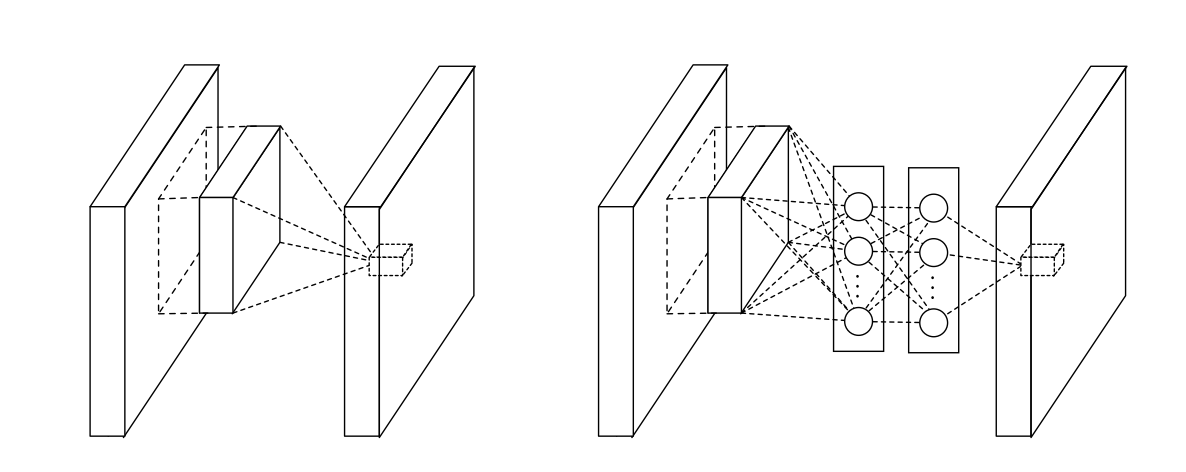
\includegraphics[scale=.6]{images/NIN.png}
\caption{Réseau Network in Network}
\label{F:NIN}
\end{figure}

Inception V1, implémenté dans le réseau GoogLeNet vainqueur d'ILSVRC 2014, est une extension à des réseaux plus profonds de Network to Network. Le réseau est composé de 22 couches et atteint 93.3\% de taux de reconnaissance. D'autres améliorations théoriques (fonctions de pertes associées aux couches intermédiaires dans la phase d'apprentissage, introduction de caractères épars dans le réseau) ont également permis d'améliorer les performances (de calcul et de classification).\\
Inception V2, puis V3 (figure  \ref{F:iv3}) adoptent des techniques de factorisation (toute convolution par un filtre de taille plus grande que 3$\times$3 peut être exprimée de manière plus efficace avec une série de filtres de taille réduite) et de normalisation pour améliorer encore les performances.\\
Inception V4 \cite{Szegedy16} propose une version rationalisée, à l'architecture uniforme et aux performances accrues.

\begin{figure}[hbtp!]
\centering
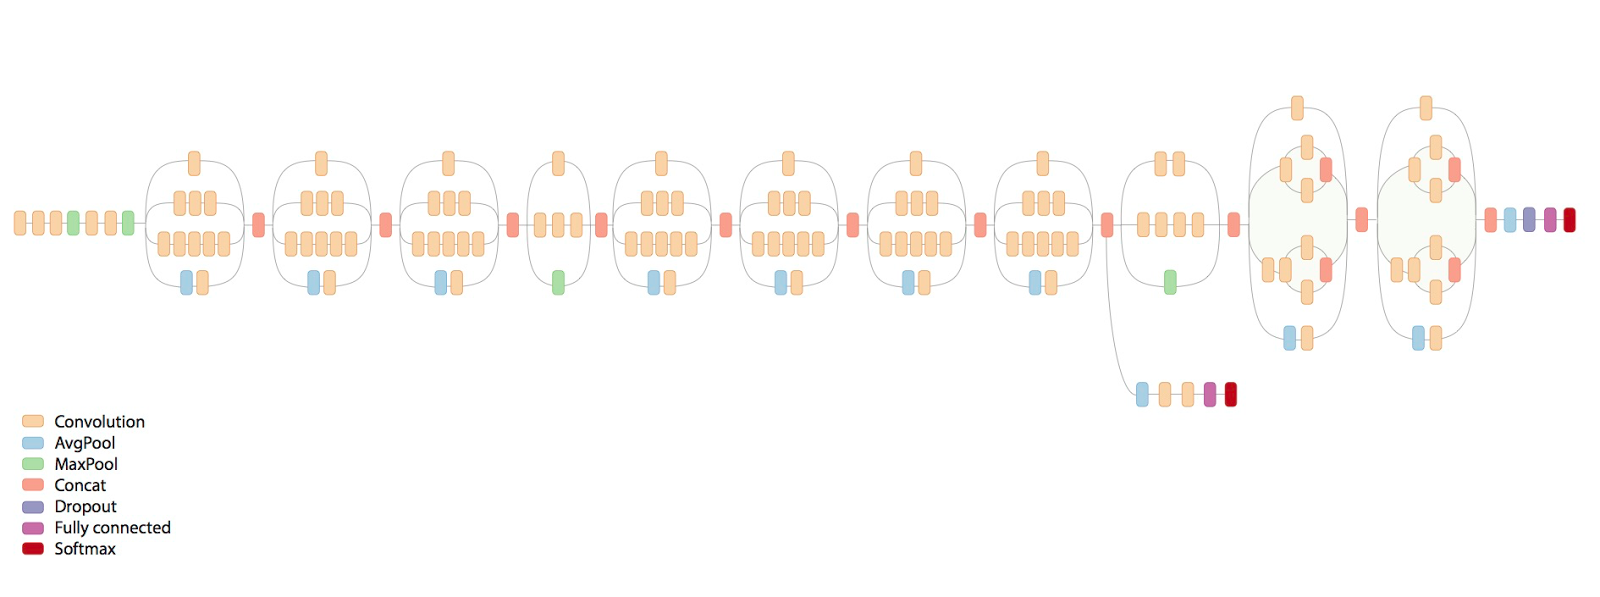
\includegraphics[width=\columnwidth]{images/inceptionv3.png}
\caption{Architecture d'inception V3}
\label{F:iv3}
\end{figure}

\subsection{ResNet}
En 2015, Microsoft remporte la compétition ILSVRC avec ResNet \cite{He15}, un réseau à 152 couches qui utilise un module ResNet. Le taux de bonne reconnaissance est de 96.4\%.  Un réseau résiduel (ou ResNet) résout le problème de vanishing gradient de la manière la plus simple possible, en permettant des raccourcis entre chaque couche du réseau. Dans un réseau classique, l'activation en sortie de couche est de la forme $y=\sigma(x)$, et lors de la rétropropagation, le gradient doit nécessairement repasser par $\sigma(x)$, ce qui peut causer des problèmes en raison de la (forte) non linéarité induite par $\sigma$. Dans un réseau résiduel, la sortie de chaque couche est calculée par $y=\sigma()+x$, où $+x$ est le raccourci entre chaque couche, qui permet au gradient de transiter directement sans passer par $\sigma$. \\
Cette représentation donne l'idée générale, mais la réalité est un peu plus complexe, et prend la forme d'un module ResNet (figure \ref{F:ResNet}).

\begin{figure}[hbtp!]
\centering
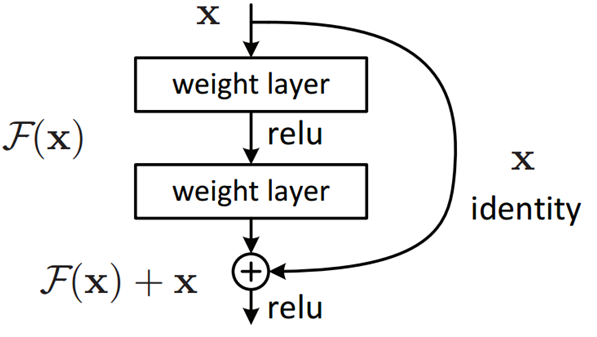
\includegraphics[scale=.37]{images/resNet.png}
\caption{Module ResNet (source : \cite{He15})}
\label{F:ResNet}
\end{figure}

\subsection{SqueezeNet}
SqueezeNet \cite{Iandola16} est un réseau produit en 2016, qui n'est pas tant remarquable par ses performances (il atteint les mêmes niveaux de reconnaissance qu'AlexNet), mais par sa légèreté (le modèle entraîné sur ImageNet a une taille de 4.9 Mo, et possède 50 fois moins de paramètres qu'AlexNet par exemple) et la rapidité avec laquelle il peut être entrainé. \\
SqueezeNet  introduit des modules "Fire" (figure \ref{F:SqueezeNet}), composés d'une couche de convolution "squeeze", dotée de filtres de taille 1$\times$1, et d'une couche d'expansion dotée de filtres de taille 1$\times$1 et 3$\times$3. L'utilisation de filtres 1$\times$1 permet une réduction du nombre de paramètres.  
\begin{figure}[hbtp!]
\centering
\includegraphics[scale=.42]{images/squeezeNet.png}
\caption{Module Fire (source : \cite{Iandola16})}
\label{F:SqueezeNet}
\end{figure}

Le réseau est composé d'une couche de convolution classique, d'une couche d'agrégation max, suivie de 9 modules Fires entrecoupées d'agrégation max, et d'une couche de convolution finale. Le nombre de filtres est progressivement augmenté entre chaque module (figure \ref{F:SqueezeNet2}).

\begin{figure}[hbtp!]
\centering
\includegraphics[width=\columnwidth]{images/squeezeNet2.png}
\caption{Architecture de SqueezeNet (source :  \cite{Iandola16})}
\label{F:SqueezeNet2}
\end{figure}


%%%%%%%%%%%%%%%%%%%%%%%
\section{Comment utiliser ces réseaux}
Il est possible de redéclarer les réseaux classiques depuis TensorFlow ou Keras, en définissant une à une les couches et leur paramètres, qui sont décrits dans les articles correspondants. On imagine assez bien le travail que cela peut représenter sur le ResNet de Microsoft...\\
Fort heureusement, il existe d'autres manières d'utiliser ces réseaux.



\subsection{Utilisation de réseaux pré-entraînés}
Il est possible avec TensorFlow  et Keras de charger / sauvegarder des réseaux qui ont été entraînés.  Il est également possible, pendant l'entraînement, de créer des sauvegardes (checkpoints) pour reprendre éventuellement l'entraînement en cours d'itérations. On peut sauvegarder tout le réseau (architecture + optimiseur  + poids), ou seulement les poids.

Pour charger / sauver les poids d'un modèle {\tt model} Keras, on utilise simplement les fonctions 
\begin{lstlisting}
model = create\_model()\\
model.load\_weights('./checkpoints/my\_checkpoint')
\end{lstlisting}
et
\begin{lstlisting}
model.save\_weights('./checkpoints/my\_checkpoint')
\end{lstlisting}

Pour charger / sauver le modèle complet, on utilise  
\begin{lstlisting}
model = keras.models.load\_model('my\_model.h5')
\end{lstlisting}
et 
\begin{lstlisting}
model = create\_model()
model.fit(xtrain, ytrain)
model.save('my\_model.h5')
\end{lstlisting}


La procédure sous Tensorflow est un peu plus complexe et est décrite \href{https://www.tensorflow.org/guide/saved_model}{ici}.


\subsection{Transfer learning et fine tuning}
Il est possible d'utiliser les réseaux classiques pré-entrainés pour de nouvelles tâches. L'idée sous-jacente et que les premières couches capturent des caractéristiques bas niveau, et que la sémantique vient avec les couches profondes. Ainsi, dans un problème de classification, où les classes n'ont pas été apprises, on peut supposer qu'en conservant les premières couches on extraira des caractéristiques communes des images, et qu'en changeant les dernières couches (information sémantique et haut niveau et étage de classification), c'est à dire en réapprenant les connexions, on spécifiera le nouveau réseau pour la nouvelle tâche de classification.\\
Cette approche rentre dans le cadre des méthodes de Transfer Learning \cite{Pan10} et de fine tuning, cas particulier d'adaptation de domaine :
\begin{itemize}
\item les méthodes de transfer learning prennent un réseau déjà entraîné, enlèvent la dernière couche complètement connectée, et traitent le réseau restant comme un extracteur de caractéristiques. Un nouveau classifieur est alors entraîné sur les caractéristiques calculées sur le nouveau problème
\item les méthodes de fine tuning ré-entrainent le classifieur du réseau, et remettent à jour les poids du réseau pré-entraîné par rétropropagation.
\end{itemize}
Plusieurs facteurs influent sur le choix de la méthode à utiliser : la taille des données d'apprentissage du nouveau problème, et la ressemblance du nouveau jeu de données avec celui qui a servi à entraîner le réseau initial : 
\begin{itemize}
\item pour un jeu de données similaire de petite taille, on utilise du transfer learning, avec un classifieur utilisé sur les caractéristiques calculées sur les dernières couches du réseau initial
\item pour un jeu de données  de petite taille et un problème différent, on utilise du transfer learning, avec un classifieur utilisé sur les caractéristiques calculées sur les premières couches du réseau initial
\item pour un jeu de données, similaire ou non de grande taille, on utilise le fine tuning
\end{itemize}
A noter qu'il est toujours possible d'augmenter la taille du jeu de données par des technique de "Data Augmentation" (changement de couleurs des pixels, rotations, cropping, homothéties, translations...)

\section{Que faire si j'ai peu de données ?}
Les m\'ethodes supervis\'ees n\'ecessitent pour de bonnes performances un ensemble d'apprentissage $\mathcal{S}$ de grand cardinal. Si seulement peu d'exemples $\mathcal{S}_s = \{(\mathbf{x}_i,y_i), i\in[\![1\cdots m ]\!]\}$ sont disponibles, avec $m$ petit, les techniques pr\'ec\'edemment d\'ecrites ne sont pour la plupart plus applicables.\\
Les m\'ethodes de Few-Shot Learning ont \'et\'e introduites pour traiter ce manque de donn\'ees. Les exemples applicatifs sont nombreux, allant de la classification d'images à l'analyse de sentiments \`a partir de textes, ou encore à la reconnaissance d'objets.  \\
Vu sous l'angle de la minimisation du risque empirique, l'hypothèse $h$ construite sur la minimisation de 
$$R(h) = \displaystyle\sum_{i=1}^m \ell(y_i,h(\mathbf{x}_i))$$
conduit à un sur apprentissage et un risque $R(h)$ très loin du risque r\'eel. Pour pallier ce probl\`eme, des connaissances \textit{a priori} doivent \^etre utilis\'ees. Le Few-shot learning propose trois alternatives. Nous détaillons ici l'une d'entre elles, l'augmentation de données.\\

Les approches de cette cat\'egorie utilisent des connaissances \textit{a priori} sur les donn\'ees pour enrichir  $\mathcal{S}_s$. On les regroupe parfois sous le vocable de m\'ethodes d'\emph{augmentation de données}.  Si elles sont faciles \`a mettre en oeuvre et \`a comprendre, ces m\'ethodes restent cependant d\'ependantes du domaine d'\'etude et ne peuvent \^etre facilement g\'en\'eralis\'ees.

Les principales strat\'egies sont r\'esum\'ees dans le tableau \ref{T:dataAug} et un exemple d'illustration est donn\'e figure \ref{Fig:dataAug}.


\begin{table}[ht!]
\renewcommand\arraystretch{2.2} 

\centering
\begin{tabular}{M{4cm}|M{2.5cm}|M{5cm}|M{2.5cm}}
\bfseries{Transformation...} & \bfseries{Entr\'ee}  & \bfseries{Op\'erateur} & \bfseries{Sortie}\\
\hline
\parbox{4cm}{... de donn\'ees de $\mathcal{S}_s$}& $(\mathbf{x}_i,y_i)\in \mathcal{S}_s$ & $t:\mathcal{X}\rightarrow \mathcal{X}$ & $(\mathbf{t(x_i)},y_i)$\\
\hline
\parbox{4cm}{... d'un ensemble de donn\'ees non \'etiquet\'ees} & $(\mathbf{x},-)$ & \parbox{5cm}{$h:\mathcal{X}\rightarrow \mathcal{Y}$ entra\^in\'e sur  $\mathcal{S}_s$}& $(\mathbf{x},h(\mathbf{x}))$\\
\hline
\parbox{4cm}{... d'un ensemble de donn\'ees similaires} & $\{(\mathbf{\hat{x}_j},\hat{y}_j)\}$ & \parbox{5cm}{Op\'erateur de combinaison $c$ }& $(c(\{\mathbf{\hat{x}_j}\}),c(\{\hat{y}_j\}))$ \\
\end{tabular}
\caption{Techniques d'augmentation de donn\'ees}
\label{T:dataAug}
\end{table}


\begin{figure}[ht!]
\centering
\includegraphics[width=\linewidth]{images/DataAugmentation}

\caption{Exemple d'augmentation de donn\'ees. De gauche \`a droite : image originale, rotation de 20$^{\circ}$, flip, ajout de bruit gaussien, déformation élastique, changement de contraste par canal RGB.} 
\label{Fig:dataAug}
\end{figure}


%%%%%%%%%%%%%%%%%%%%%%%
\section{Partie pratique}
Vous avez à disposition un notebook vous proposant d'apprendre, à partir d'un réseau pré-entrainé (\href{https://arxiv.org/abs/1801.04381}{MobileNetV2}, assez léger et performant en classification), de fine-tuner ce dernier pour un problème où les données ne font pas partie de la base d'entraînement initiale (l'objectif ici est d'apprendre à classifier des fleurs en 5 catégories). Votre travail consiste à :
\begin{itemize}
\item Appliquer une technique d'augmentation de données pour augmenter le nombre d'images de fleurs. Pour ce faire, vous utiliserez l'objet \href{https://www.tensorflow.org/api_docs/python/tf/keras/preprocessing/image/ImageDataGenerator}{ImageDataGenerator}, que nous vous laissons prendre en main...
\item Créer le modèle. vous chargerez  tout d'abord le réseau MobileNetV2 (fonction \href{https://www.tensorflow.org/api_docs/python/tf/keras/applications/MobileNetV2}{MobileNetV2}). Vous supprimerez ensuite la dernière couche de ce réseau (la couche de classification) à l'aide de la fonction \href{https://keras.io/guides/sequential_model/}{pop}, puis ajouterez votre propre couche de classification. Vous indiquerez  ensuite quels poids ne doivent pas être réappris (en taggant les couches correspondantes avec le drapeau \texttt{layer.trainable = False}), et réentrainerez le nouveau réseau sur la nouvelle base augmentée. Vous pourrez tester l'influence du nombre de couches non réentrainées.
\item Evaluer la précision de votre réseau.
\end{itemize}


\bibliographystyle{plain}
\bibliography{../../biblio}
\end{document}
